%
% File: chap01.tex
% Author: Victor F. Brena-Medina
% Description: Introduction chapter where the biology goes.
%
\let\textcircled=\pgftextcircled
\chapter{Experimental Results}
\label{chap5}
\initial{T}he performance of the classifications and detections is significantly determined by the pre-processing of training data,  the hyper-parameters of the network and the training parameters. A number of experiments are performed to demonstrate how those factors influence the performance. We start off with the results of how the pre-processing of training data and the hyper-parameters of the network affect the classification accuracy base on a singleNet, see \ref{tuning_network}. At last, we give the overall experimental results of the classification and detection tasks.
  
\section{Searching of the optimal parameters}
We first introduce the network model which we employ for searching of the optimal parameters.  Then, we will overall introduce the factors which would affect the classification accuracy. Finally, we present the experimental schemes, results and analyses. 
\subsection{Model}
\label{tuning_network}
Due to limitation of GPU memory and training time, we search the optimal parameters of the data pre-processing and the network on a singleNet which is only composed by a global interaction feature descriptor instead of the hierarchical interaction feature descriptor and a softmax classifier. The architecture of the singleNet is illustrated in Figure \ref{fig:arch_eval}. We assume that if the parameters are optimal for the singleNet, then they are also optimal parameters for the fullNet which is composed by the hierarchical interaction feature descriptor and a softmax classifier, see Section \ref{arch_classification},  because they have similar network model.  
 \begin{figure}
 	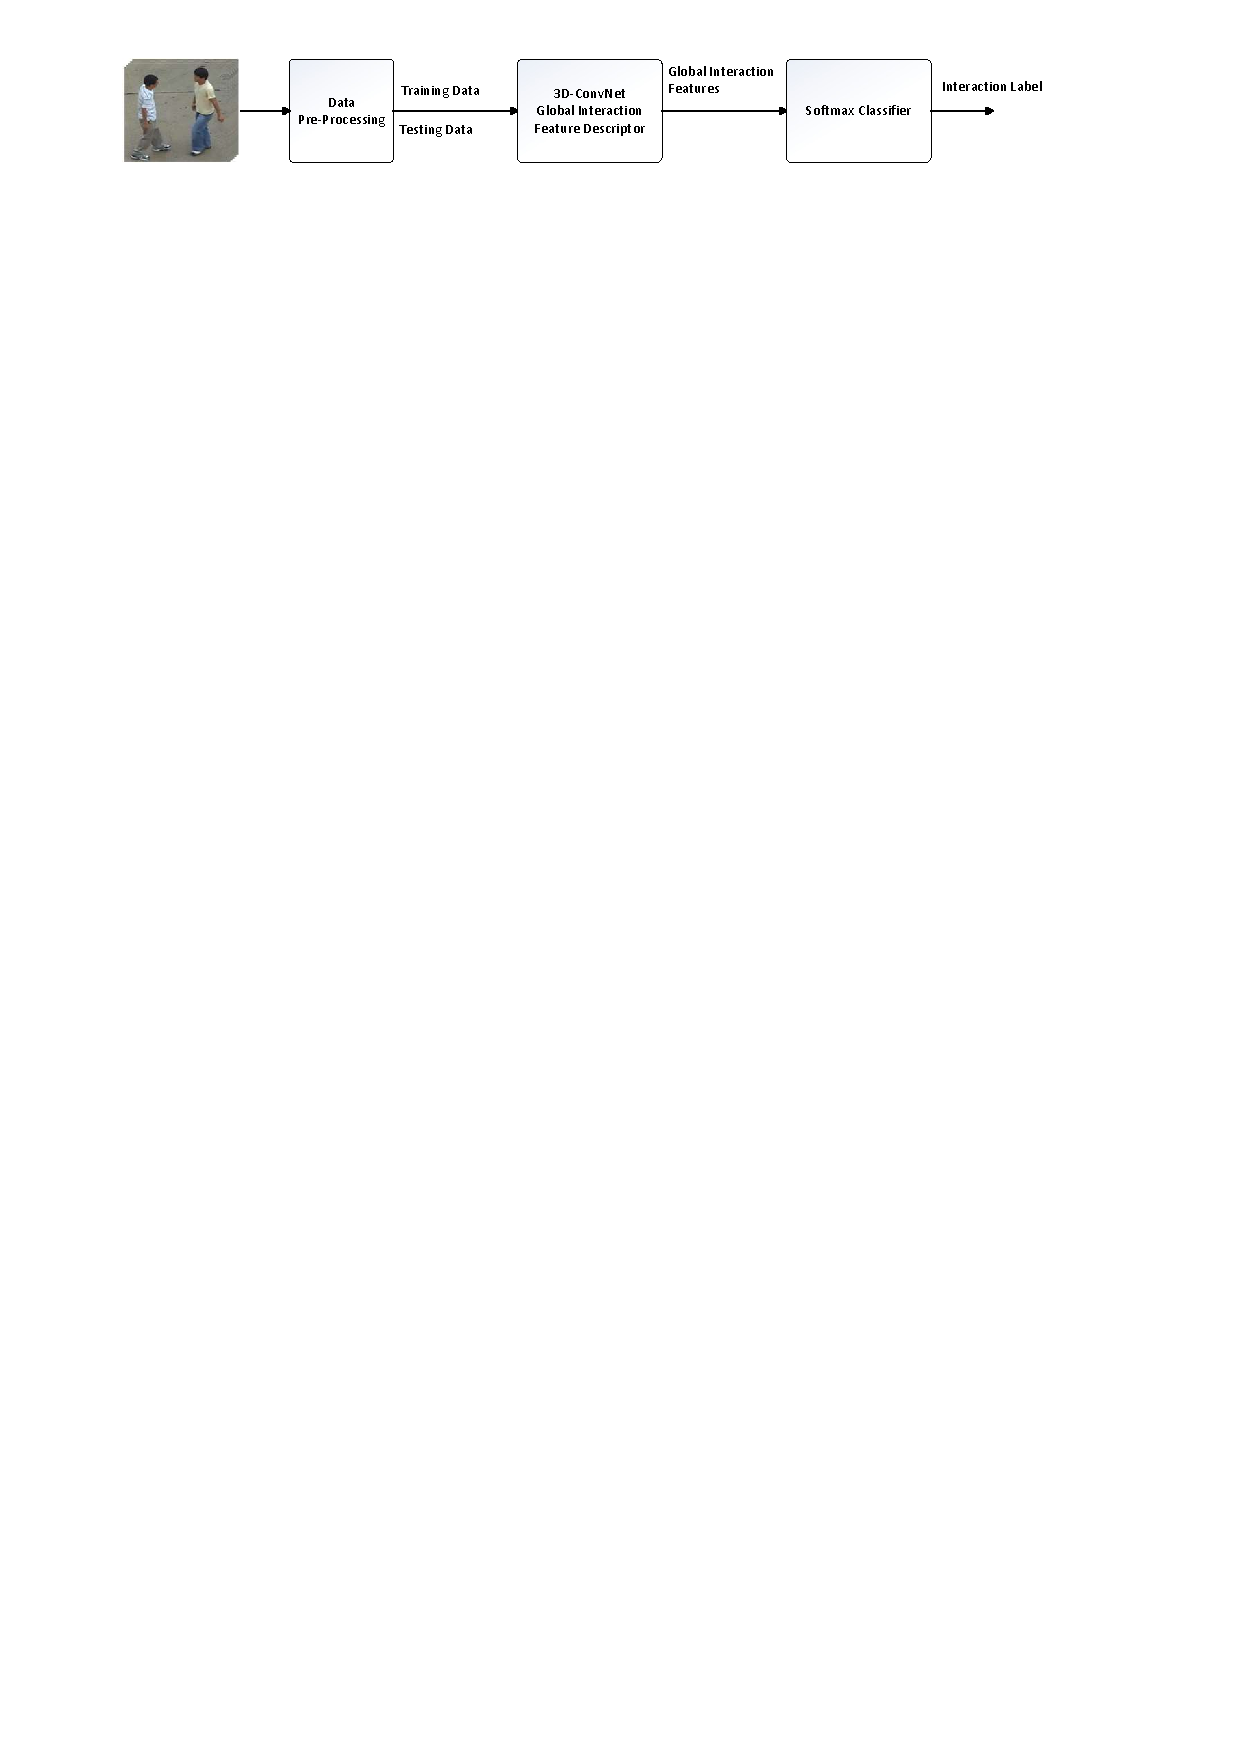
\includegraphics[trim=2cm 26.5cm 0cm 1cm]{fig01/arch_eval.pdf}
 	\caption{The architecture of the singleNet}
 	\label{fig:arch_eval}
 \end{figure}
Due to that we only need to search the optimal parameters by comparing the loss and classification accuracy between different parameter settings, it is not necessary to evaluate them on all data. For the sake of saving training time, it is reasonable to use part of data instead of the all. So, all training and testing video used in the experiments of this section are from the UT-Interaction dataset set1, see Section \ref{ut-interaction}.  

\subsection{Assumptions and Factors and the default parameter setting}
Since there are many factors which influence the classification accuracy, and many parameters in each factor, it is impossible to search the optimal parameters by going through all the model parameters, at least under our current resource conditions. So, we assume that the effects of each parameter on the classification accuracy are independent. Based on this assumption, we have a set of default parameters as shown in Table \ref{table:default_paras}. We only adjust the parameters of one factor, keep the other parameters as default value, and observe the experimental results. At last, we use the combination of each factor's optimal parameter as our network's optimal parameters.
  \renewcommand\arraystretch{1.2}  
  \begin{table}
  	\caption{Default parameters for network and data pre-processing}
  	\begin{center}
  		\begin{tabular}{| m{0.6cm} | m{7cm} | m{6cm} |}
  			\hline
  			\textbf{No.} & \textbf{Factors} & \textbf{Parameters}  \\ \hline \hline
  			% Network
  			\multicolumn{3}{|l|}{\textbf{Network}}  \\ \hline
  			
  			1 & Initial values of the network parameters, see Section \ref{Initialization}. & \tabincell{l} 
  						{\(weights = N(0,\sigma^2)\), \(\sigma = 0.01\) \\ 
  						 \(biases = 0 \)} \\ \hline
  			
  			2 & Dynamic adjusting of the learning rate, see Section \ref{learning_rate}. & \(Learning\ rate = 1e^{-4} \times 2^{-int(\frac{epoch}{4})} \)	\\ \hline
  			
  			3 & Dropout layers, see Section \ref{dropout} & \(keep\_ratio = 0.5\)	\\ \hline
  			
  			4 & Batch normalization layers, see Section \ref{bn} &  Yes  \\ \hline
  			
  			5 & The number of convolutional layers, see Section \ref{3dconv_layers} & 4\\ \hline
  			
  			6 & The size of convolutional kernels, see Section \ref{3dconv_filters} & \(3 \times 3 \times 3\) \\ \hline
  			
  			7 & The sizes of the pooling kernels, see Section \ref{3dconv_filters} & \tabincell{l}
  			                                       {L1: \(1 \times 2 \times 2 \) \\ 
  			                                       	L2, L3: \(2 \times 2 \times 2 \) \\
  				                                    L4: \(4 \times 2 \times 2 \)}   \\ \hline
  			                                    
  			8 &  The number of filters for each convolutional layer, see Section \ref{3dconv_filters} &  \tabincell{l}
  														{nof\_conv1 = 32 \\ 
  														nof\_conv2 = 128 \\
  														nof\_conv3 = 256 \\
  														nof\_conv4 = 512}   \\ \hline
  													
  			9 &  The number of output neurons for each fully connected layer, see Section \ref{fc} & \(\text{noo\_fc}_*\) = 4096 \\ \hline \hline                           
  			
  			% Network
  			\multicolumn{3}{|l|}{\textbf{Data pre-processing}}  \\ \hline
  			1 & Data augmentation: horizontal flipping, see Section \ref{pre_processing} \ref{augmentation} & Yes  \\ \hline
  			2 & Data augmentation: random cropping, see Section \ref{pre_processing} \ref{augmentation} & Yes, 4 times \\ \hline
  			3 & Temporal down-sampling of frames, see Section \ref{pre_processing} \ref{down-sampling} & Yes, N=0, see \ref{down-sampling} \\ \hline

  			4 & Data normalization, see Section \ref{pre_processing} \ref{normalization} & Yes, \(X_i = \frac{X_i - Mean(X)}{Std(X)}\) \\ \hline			
  		\end{tabular}
  		\label{table:default_paras}
  	\end{center}
  \end{table} 
   
\subsection{Experiments}
%***********************************************
% initializations
%**********************************************
\subsubsection{Initialization of the network parameters}
\paragraph{Experimental scheme}
To observe how much the initial values of the weights affect the classification accuracy,  we evaluated two initialization methods, including normal distribution with zero mean  and "Xavier" method \cite{xavier}. We evaluated the "Xavier" initialization with uniform distribution to compare the performance between the two main-stream initialization schemes. We initialize all biases to \(0.1\) when we evaluate the weights initializations.
\par 
It's possible and common to initialize the biases to zero, but we only tested non-zero initial biases  because we use ReLU non-linearities and non-zero initialization of biases ensures that all ReLU units fire in the beginning and therefore obtain and propagate some gradient. We evaluated 3 constant value initializations for biases, including 0,001, 0.01 and 0.1. 

\paragraph{Experimental results and analysis}
 
The experimental results of comparison between "Xavier" and normal distribution initialization (\(\mu = 0, \sigma = 0.1\)) are illustrated in Figure \ref{fig:plot_xavier_vs_normal}.  The experimental results of the three different initial biases are illustrated in Figure \ref{fig:plot_biases}. 

\begin{figure}
	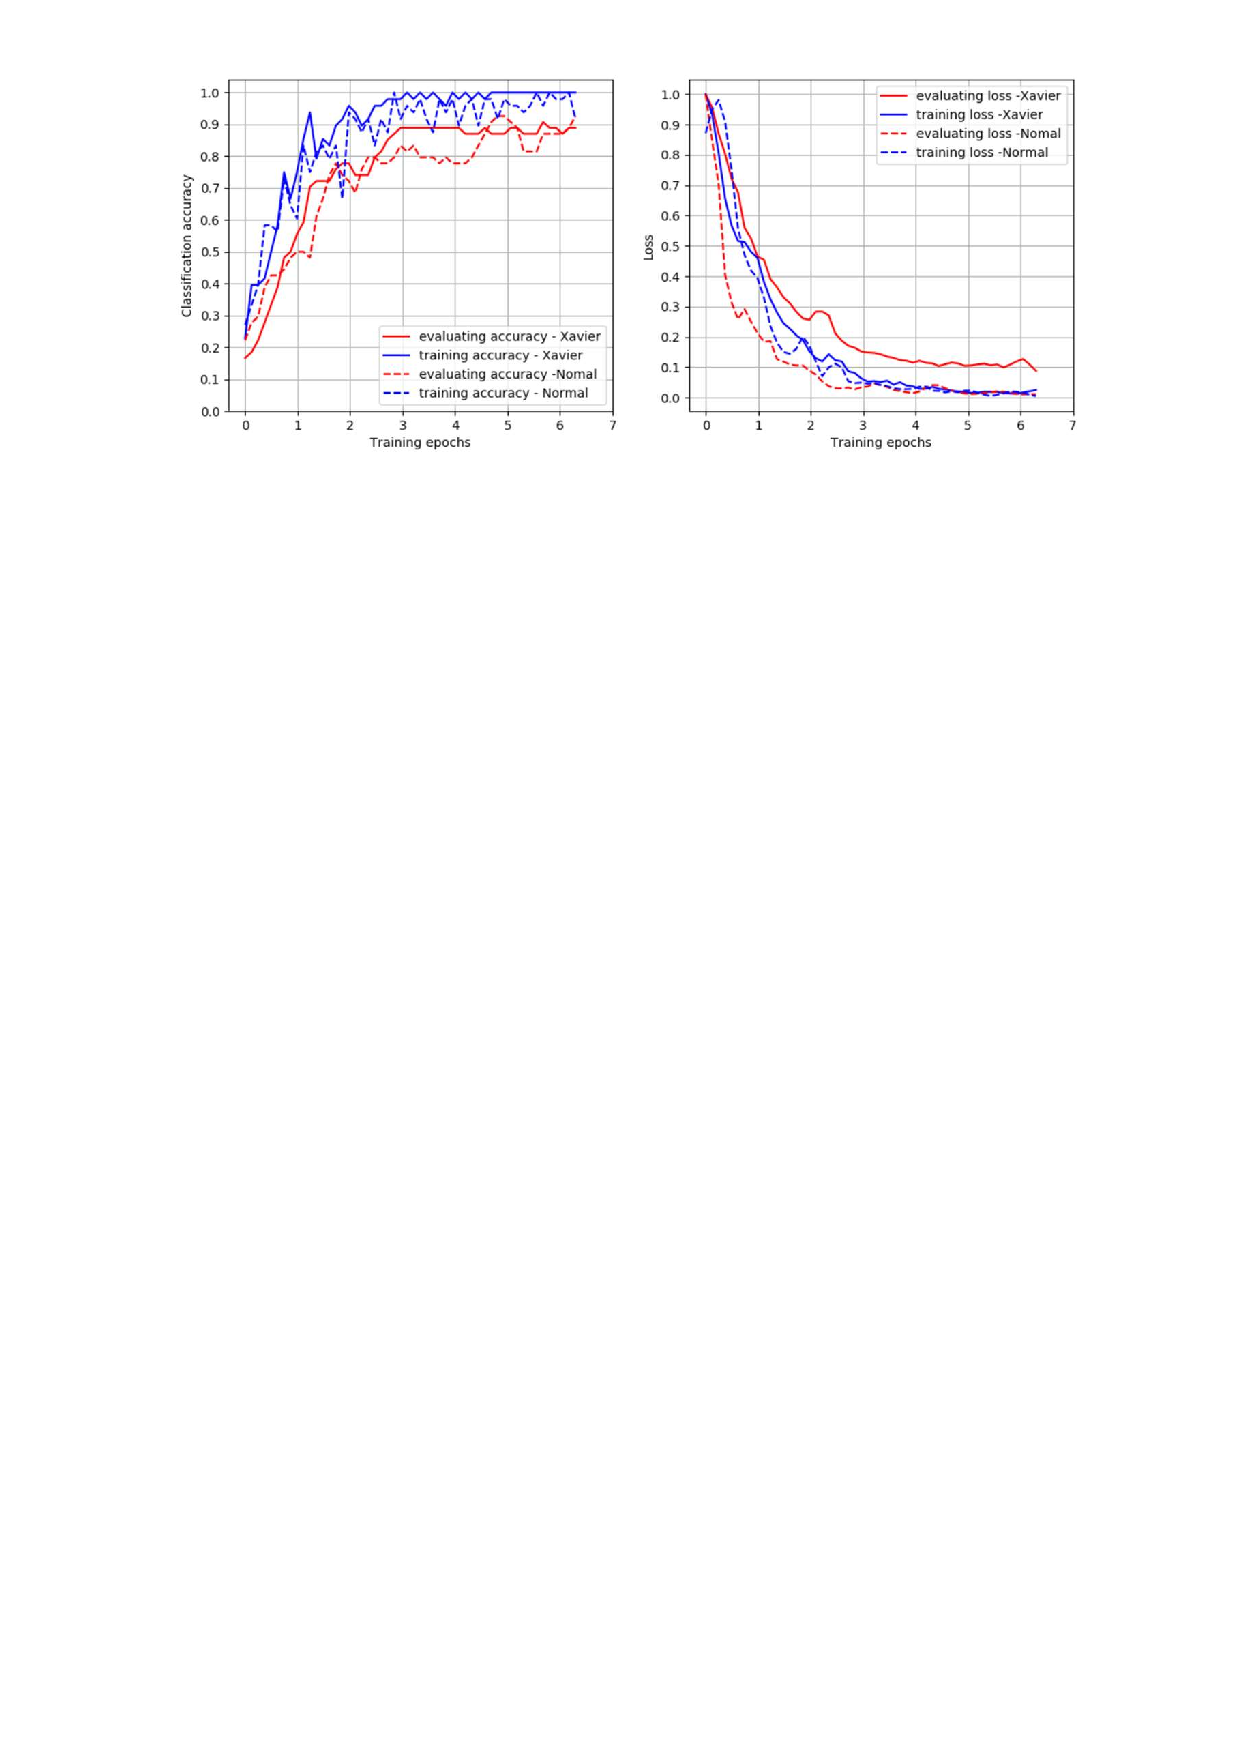
\includegraphics[trim=3cm 22cm 0cm 1cm]{fig01/plot_xavier_vs_normal.pdf}
	\caption{The loss and classification accuracy vs. training epochs comparison between "Xavier" and normal distribution initialization.}
	\label{fig:plot_xavier_vs_normal}
\end{figure}

 \begin{figure}
	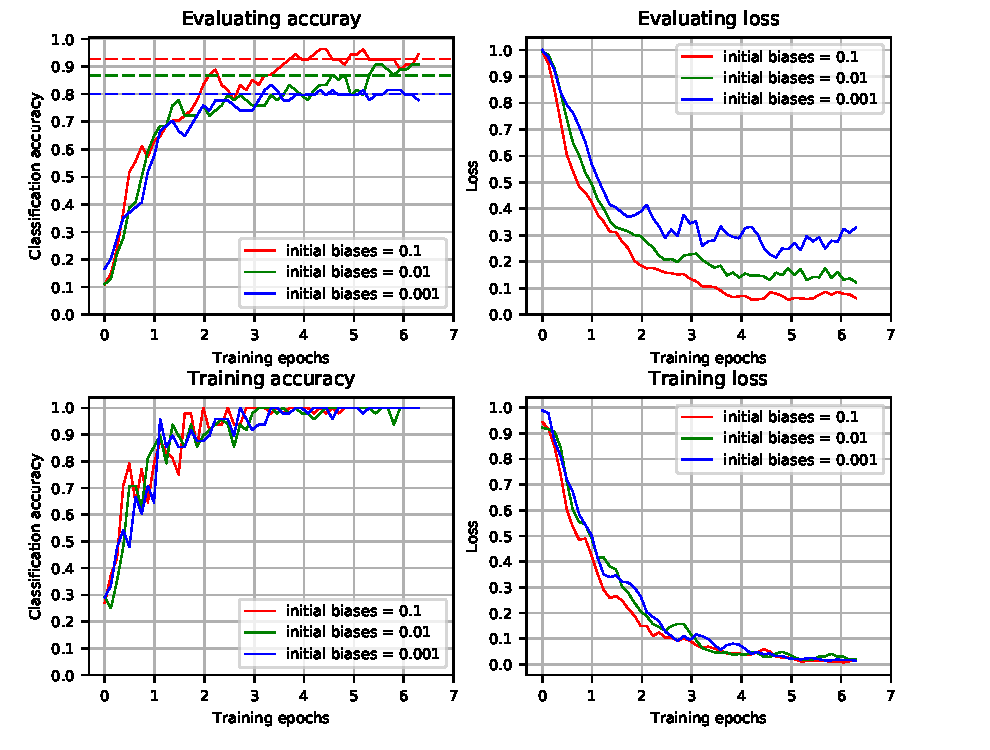
\includegraphics[trim=0cm 0cm 0cm 0cm]{fig01/plot_biases.pdf}
	\caption{The loss and classification accuracy vs. training epochs comparison between different initial biases.}
	\label{fig:plot_biases}
\end{figure}

From the experimental results, we can get following conclusions about the initializations of network parameters (weights and biases): 
\begin{enumerate}
	\item Under the same network condition, "Xavier" initialization gets more stable classification accuracy that the normal distribution initialization. 
	\item The evaluating loss of the "Xavier" initialization is slight larger that that of the normal distribution initialization. But this may be caused by the far larger initial loss value of the normal distribution initialization. There is no obvious over-fitting for both initializations.
	\item For the initialization of biases, network with relative larger initial biases can converge faster and achieve better classification accuracy with the ReLU non-linearity.
\end{enumerate} 
So, we will employ "Xavier" initialization in our network and set the initial biases to 0.1. 
%***********************************************
% learning rate
%***********************************************
\subsubsection{Learning Rate}
\paragraph{Experimental scheme}
We tested both constant learning rate and decaying learning rate over the period of the training process.  For constant learning rate, we tested values including 0.001, 0.0001 and 0.00001. We also tested the case that the learning rate is divided by 2 after every 3 epochs with initial value 0.0001.
 
\paragraph{Experimental results and analysis}
The experimental results of the loss and classification accuracy vs. training epochs comparison between networks with different learning rate are illustrated in Figure \ref{fig:plot_lr}.
 \begin{figure}
	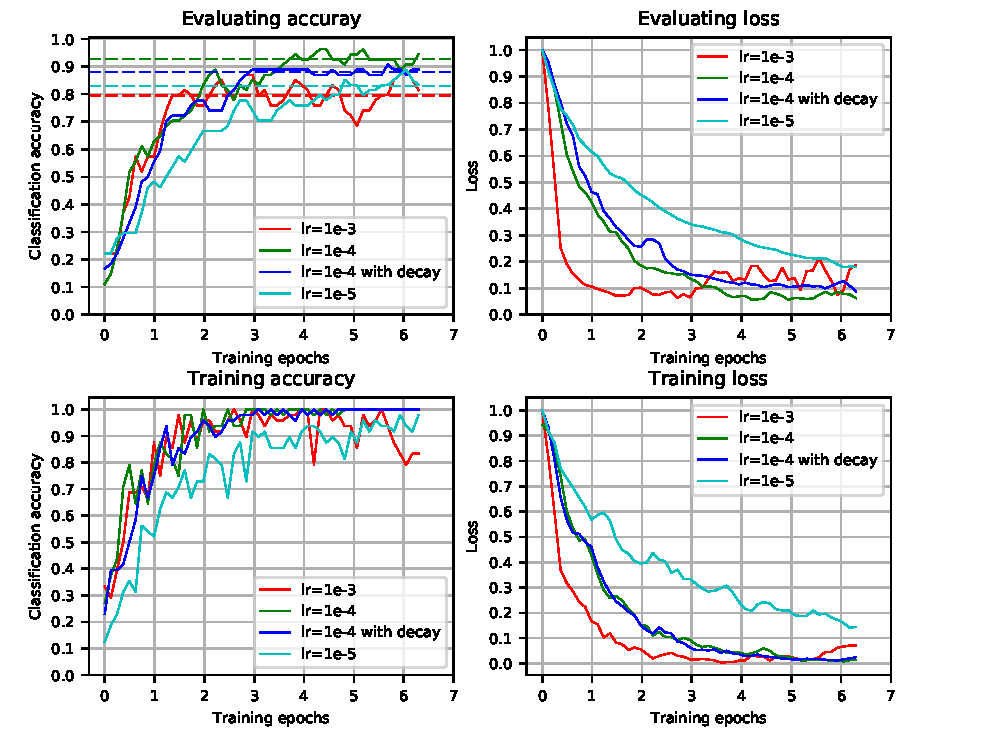
\includegraphics[trim=0cm 0cm 0cm 0cm]{fig01/plot_lr.pdf}
	\caption{The loss and classification accuracy vs. training epochs comparison between networks with different learning rate.}
	\label{fig:plot_lr}
\end{figure}
According to the experimental results, we can get following conclusion about the learning rate:
\begin{enumerate}
	\item Larger learning rate, e.g. \(1e-3\), accelerates the convergence speed of the network, but it is also easier to over-fit to the training data and even causes unstability.
	\item The training process with smaller learning rate, e.g. \(1e-5\), converge slowly. 
	\item The training processes with learning rate \(1e-4\) is more suitable for our network. And whether decay the learning rate over to the training epochs doesn't affect the performance much.   
\end{enumerate}
So, we set the learning rate to \(1e-4\) for our network.

%***********************************************
% dropout
%***********************************************
\subsubsection{Dropout layer}
\paragraph{Experimental scheme}
Dropout layer is considered as an extremely effective way to reduce overfitting in neural network,see Section \ref{fc}. We tested different values of the probability \(p\), including 0.8,0.5,0.2.

\paragraph{Experimental results and analysis}
The experimental results of the loss and classification accuracy vs. training epochs comparison between different keep probabilities of the dropout layers are illustrated in Figure \ref{fig:plot_dropout}.
\begin{figure}
	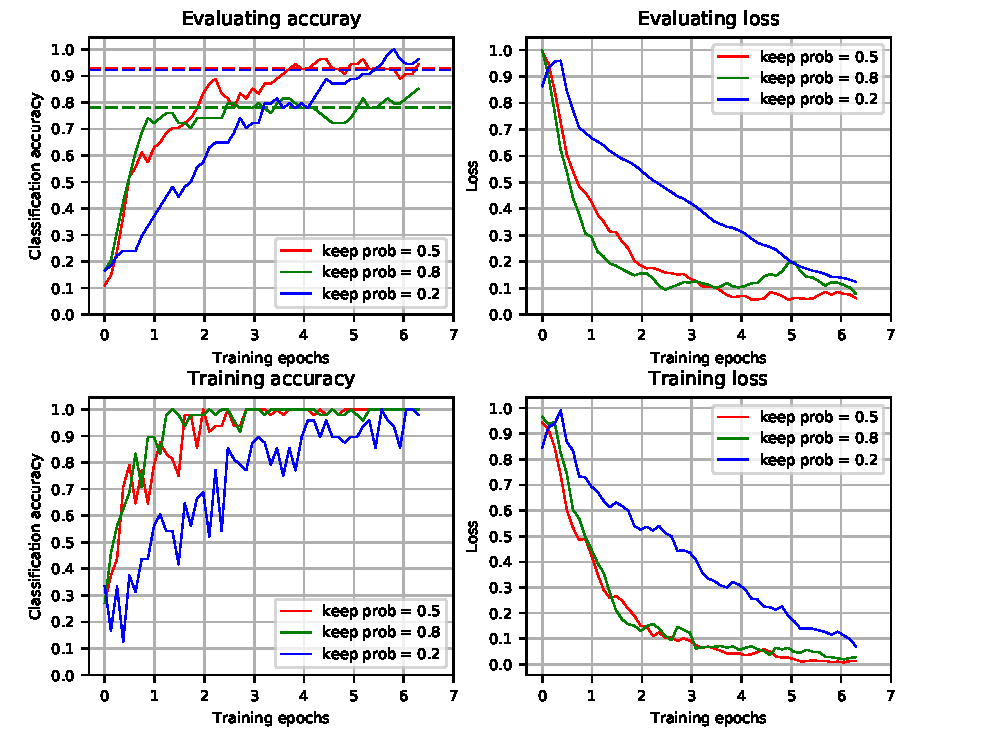
\includegraphics[trim=0cm 0cm 0cm 0cm]{fig01/plot_dropout.pdf}
	\caption{The loss and classification accuracy vs. training epochs comparison between different keep probabilities in the dropout layers.}
	\label{fig:plot_dropout}
\end{figure}

According to the experimental results, we can get following conclusion about the keep probabilities in the dropout layers:
\begin{enumerate}
	\item Larger keep probability (0.8) in the dropout layers makes the network converge faster, but the classification accuracy keeps at a lower level after convergence.
	\item Smaller keep probability (0.2) in the dropout layers makes the network converge slower, but the final classification accuracy is higher after convergence.
	\item 0.5 is a reasonable value of keep probability because it has good balance between performance and convergence speed.
\end{enumerate}
So, we set the keep probabilities to 0.5 in our network. 

%***********************************************
% batch normalization
%***********************************************
\subsubsection{Batch normalization layer}
\paragraph{Experimental scheme}
To observed the effects of batch normalization (BN) layers, see Section \ref{bn}, we compared the loss and classification accuracy between the network with and without BN layers. The only difference between the two networks is whether there are BN layers after the first two ReLU layers.  

\paragraph{Experimental results and analysis}
The experimental results of the loss and classification accuracy vs. training epochs comparison between networks with and without Batch normalization layers are illustrated in Figure \ref{fig:plot_bn_en}.
 \begin{figure}
	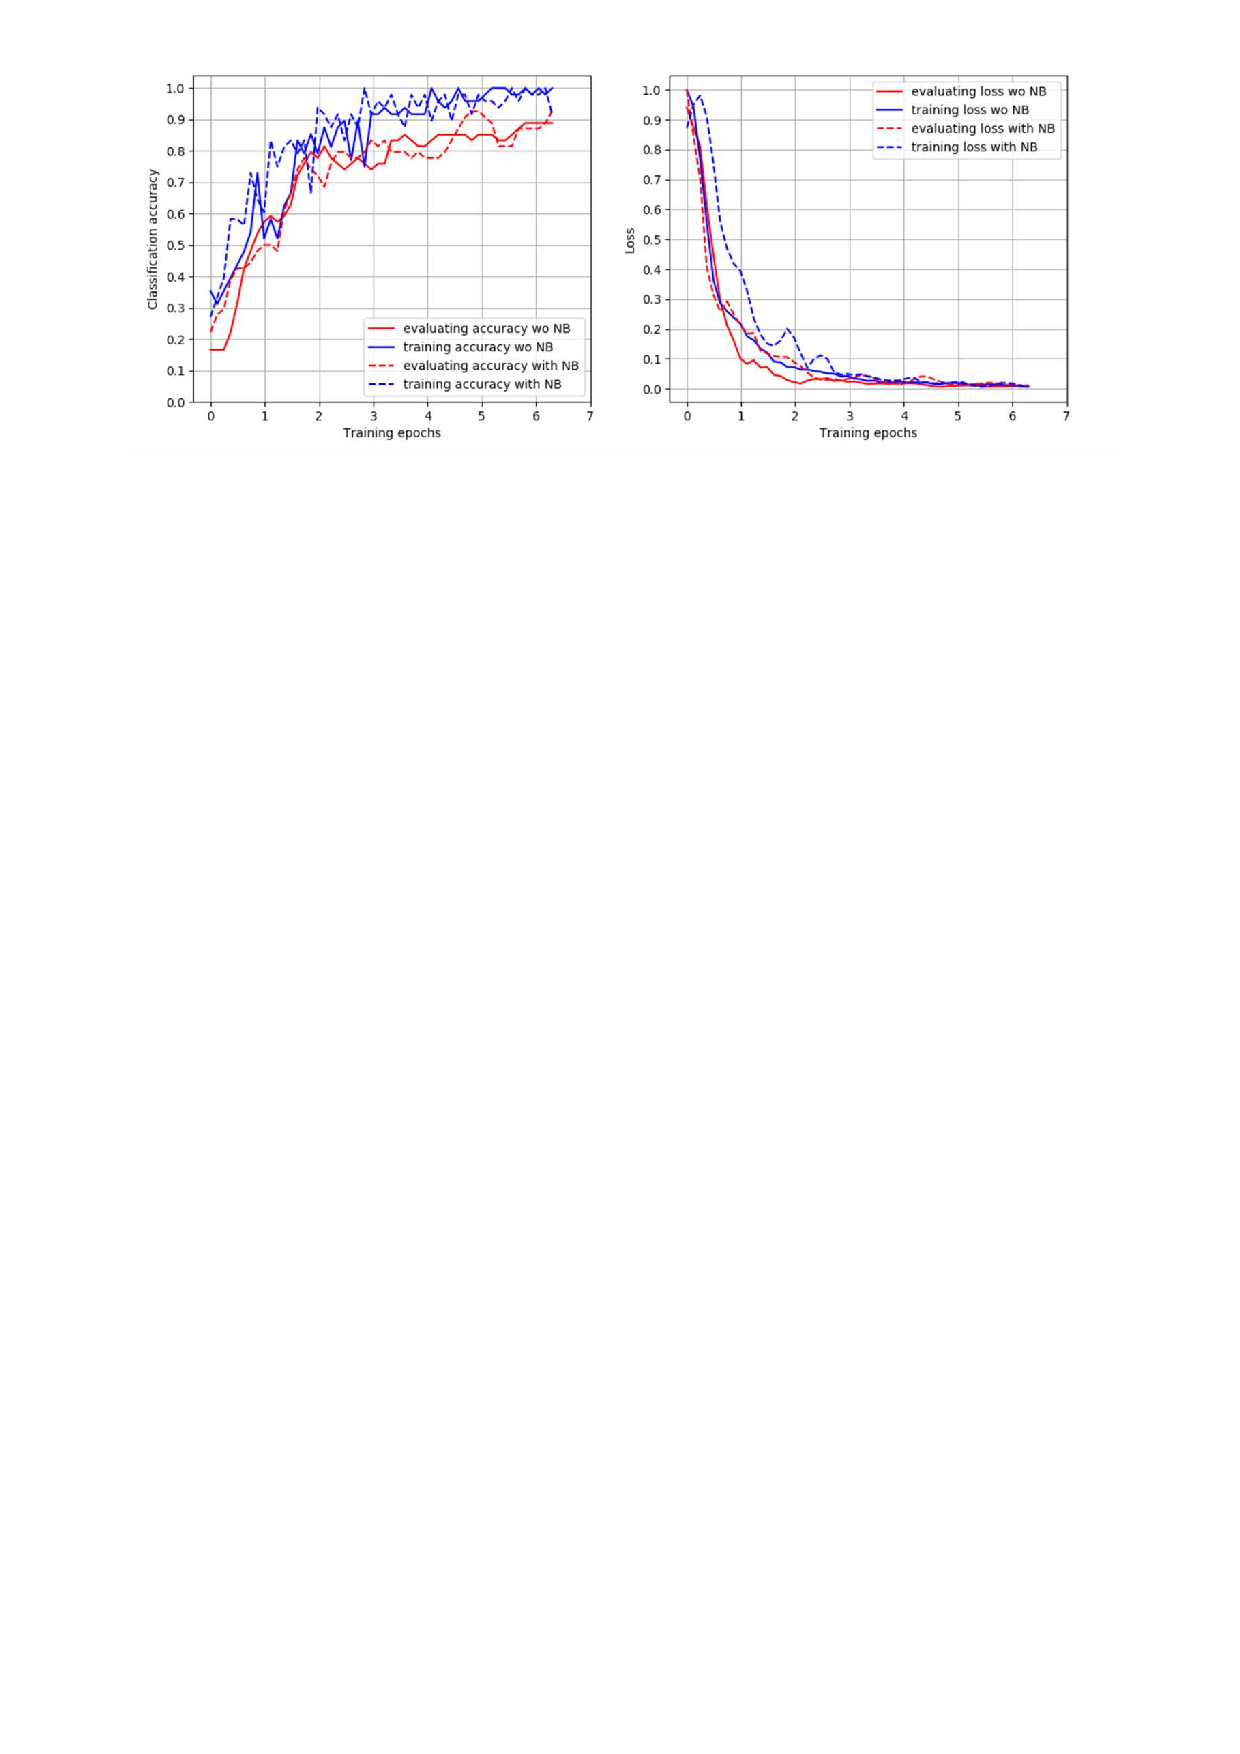
\includegraphics[trim=2.5cm 22.5cm 0cm 1cm]{fig01/plot_bn_en.pdf}
	\caption{The loss and classification accuracy vs. training epochs comparison between networks with and without batch normalization layers.}
	\label{fig:plot_bn_en}
\end{figure}

According to the experimental results, we can get following conclusions about batch normalization layers: 
\begin{enumerate}
	\item The convergence speed comparison between the network with and without BN layers is similar.
	\item The network with batch normalization layers gets slightly higher classification accuracy, about 0.92, that the network without batch normalization layers, about 0.88.
\end{enumerate}
So, we add batch normalization layers in our network. 

%***********************************************
% the number of convolution layers
%***********************************************
\subsubsection{The number of the convolutional layers}
\paragraph{Experimental scheme}
Generally, the network can get stronger global information representing ability and nicer non-linearity by applying multiple convolutional layers. In our project, we tested 3 networks with different number of 3D convolutional layers, 4, 5 and 6, respectively. The structures and parameters of the three network are illustrated in Figure \ref{fig:cnn_layers}.
\begin{figure}
 	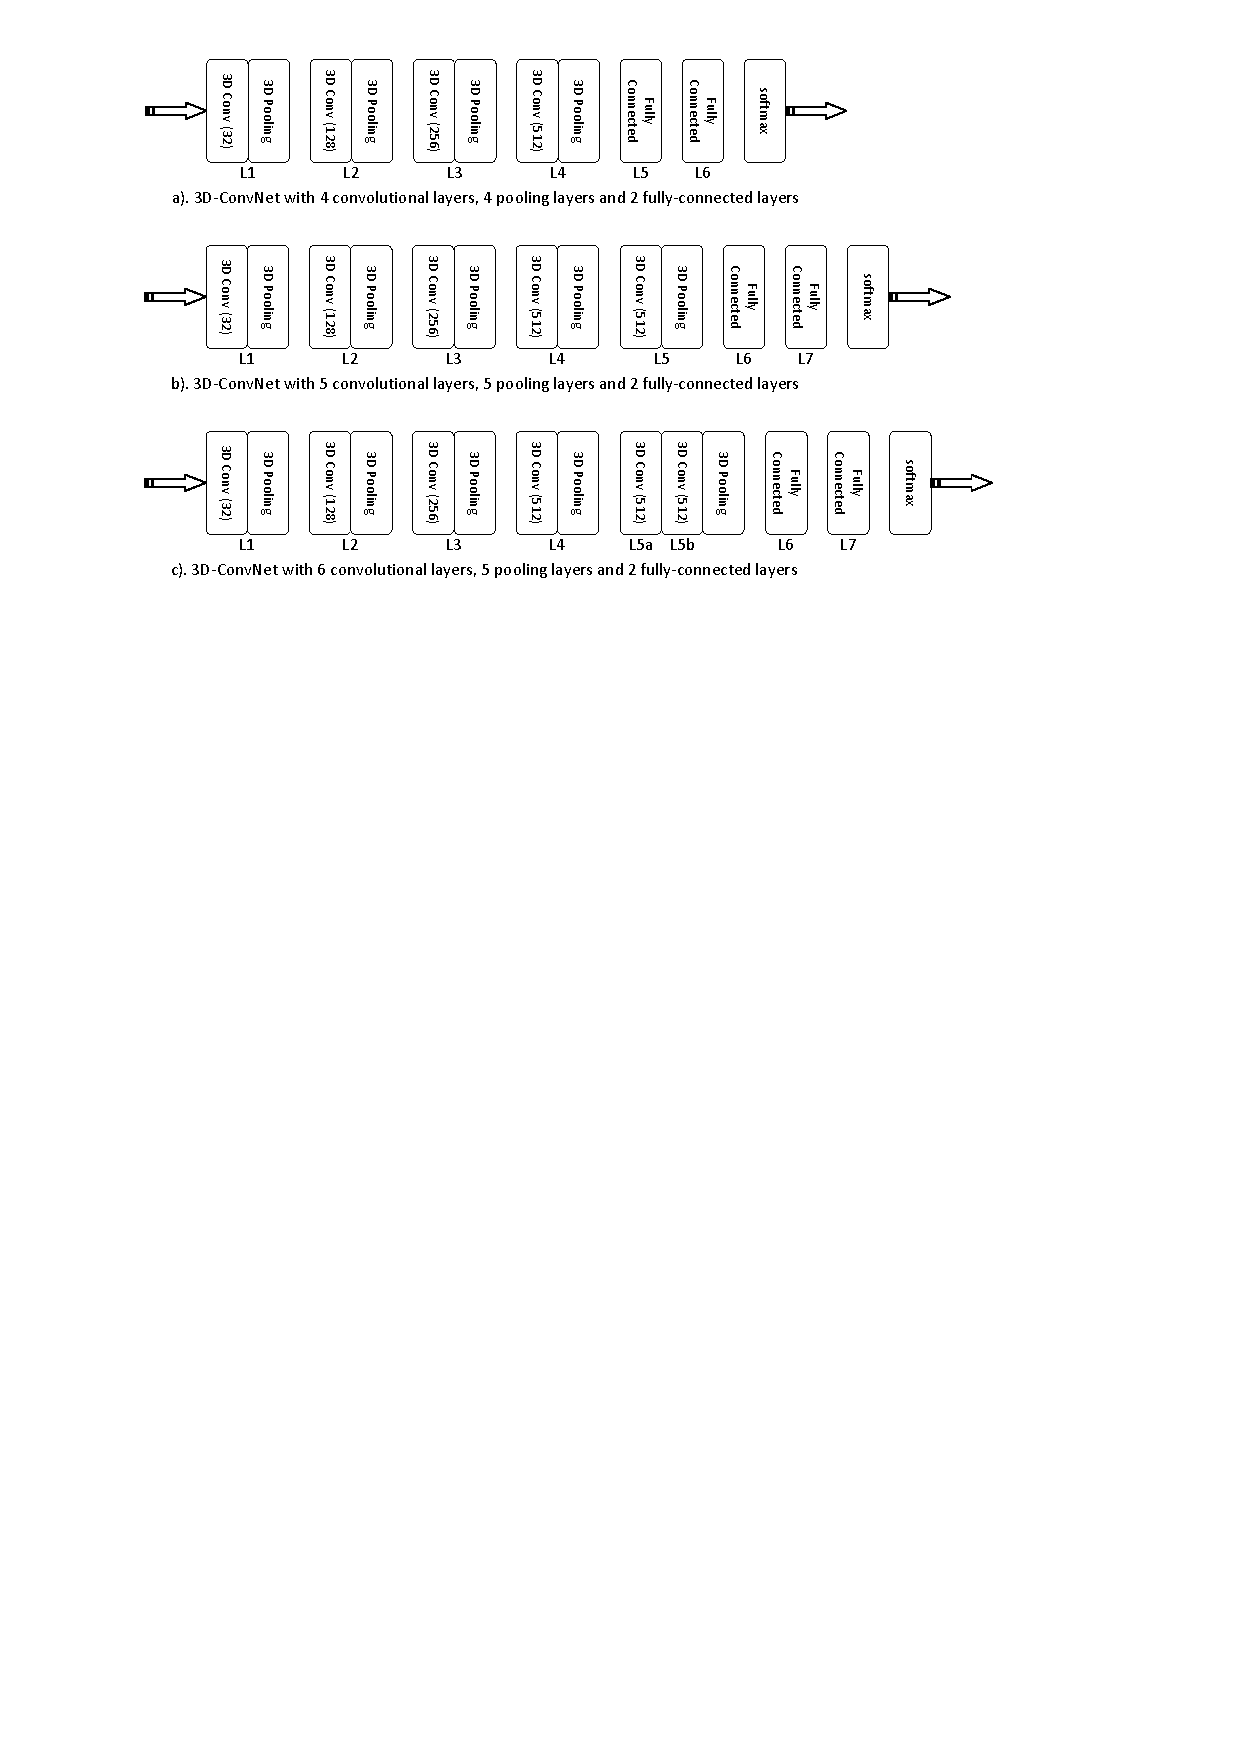
\includegraphics[trim=1cm 20cm 0cm 1cm]{fig01/cnn_layers.pdf}
 	\caption{The structures and parameters of the three 3DConvNets which have different number of convolutional layers.}
 	\label{fig:cnn_layers}
\end{figure}
\paragraph{Experimental results and analysis}
According to the experimental results, as shown in Figure \ref{fig:plot_layers}, we can get following conclusions about the different number of the 3D convolutional layers: 
\begin{enumerate}
	\item The convergence speed is not affected by the number of the 3D convolutional layers.
	\item The 3DConvNet with 5 convolutional layers gets the best classification accuracy among the three. This may be caused by that the more layers the stronger global information representing ability. But at the same time, the network with more layers also need to be trained on richer training data, else, it may perform even worse, e.g. the case of the 3DConvNet with 6 convolutional layers.
\end{enumerate}
\begin{figure}
	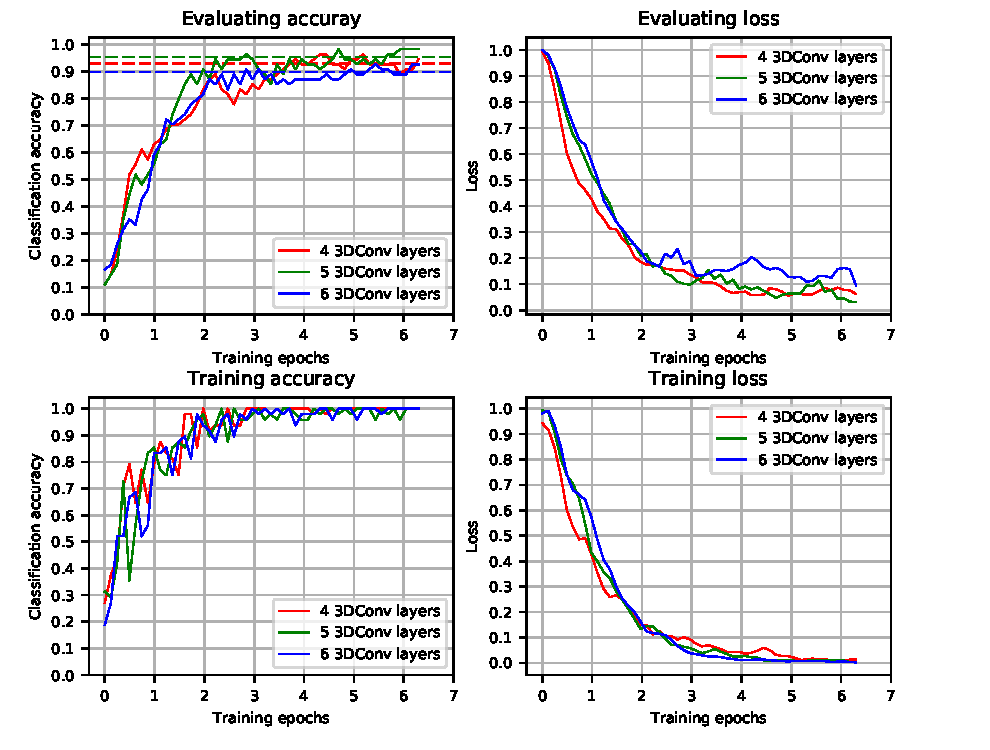
\includegraphics[trim=0cm 0cm 0cm 1cm]{fig01/plot_layers.pdf}
	\caption{The loss and classification accuracy vs. training epochs comparison between networks with different convolutional layers.}
	\label{fig:plot_layers}
\end{figure}

So, we set 5 convolutional layers in our 3DConvNet.


%***********************************************
% the size of the convolutional kernel
%***********************************************
\subsubsection{The size of the convolutional kernel}
\paragraph{Experimental scheme}
We evaluate how much does the performance relate to the size of convolutional kernels by comparing four networks with different convolutional kernel sizes, including \(3 \times 3 \times 3\), \(3\times 4 \times 4\), \(4\times4\times4\) and \(4\times 4 \times 3\), see Section \ref{3dconv_filters} for the format of kernel size. We set all convolutional layers share the same kernel size in each 3DConvNet. 

\paragraph{Experimental results and analysis}
According to the experimental results, as shown in Figure \ref{fig:plot_cnn_kernel}, we found that there is no obvious difference both in the convergence speed and classification accuracy among the networks with different convolutional kernel sizes. So, we keep to use the the size of \(3\times 3 \times 3\) for all convolutional kernels.
\begin{figure}
	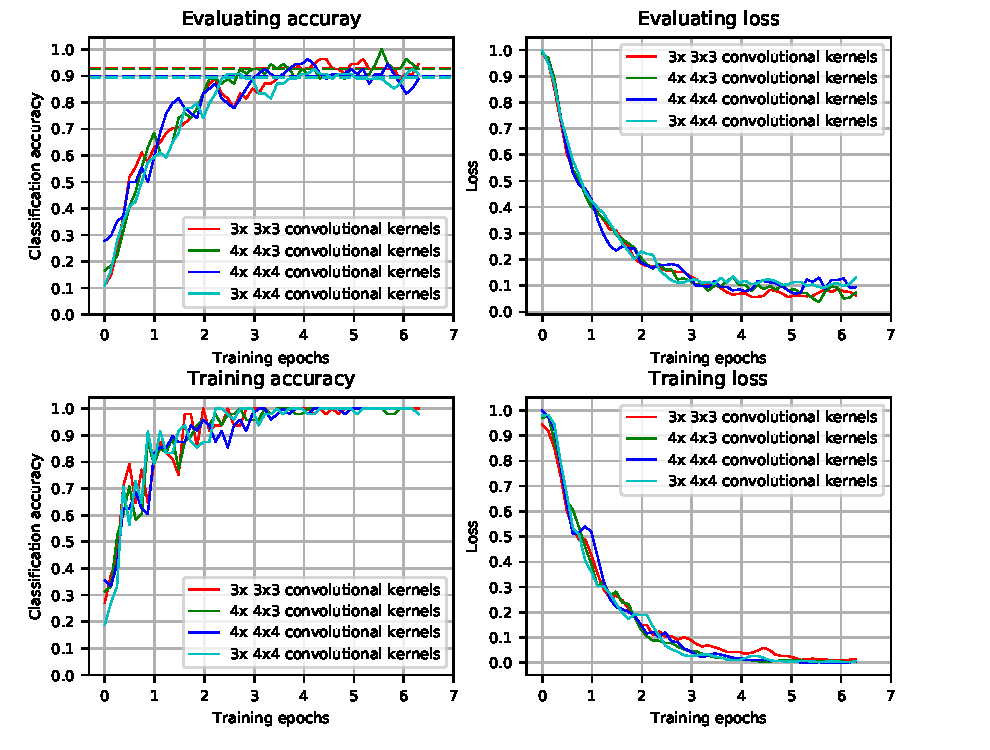
\includegraphics[trim=0cm 0cm 0cm 0cm]{fig01/plot_cnn_kernel.pdf}
	\caption{The loss and classification accuracy vs. training epochs comparison between networks with different sizes of the convolutional kernels.}
	\label{fig:plot_cnn_kernel}
\end{figure}


%***********************************************
% The number of filters for each convolutional layer
%***********************************************
\subsubsection{The number of filters of each convolutional layer}
\paragraph{Experimental scheme}
We use a 3DConvNet with 4 convolutional layers to evaluate the relationship between the performance and the number of filters of each convolutional layer. We performed four experiments which adjust the number of filters for only one convolutional layer each time, including 1). \(nof\_conv1\ 32 \rightarrow 64\), 2). \(nof\_conv2\ 128 \rightarrow 64\), 3). \(nof\_conv3\ 256 \rightarrow 512\), and 4). \(nof\_conv4\ 512 \rightarrow 256\).

\paragraph{Experimental results and analysis}
The experimental results are illustrated in the Figure \ref{fig:plot_nof}. The numbers listed in the legend represent the numbers of the filters for each convolutional layer, e.g. \([32,128,256,512]\) represents \(nof\_conv1 = 32, nof\_conv2 = 128, nof\_conv3 = 256, nof\_conv4 = 512\). 
\par 
According to the experimental results, the networks perform a little better when the numbers of the filters are  \([32,128,256,512]\) and \([32,128,512,512]\), while the performance is a little worse when the numbers of the filters are \([32,64,256,512]\).
It is hard to the find the potential laws and explain why they perform better or worse from the limited experimental data. We just use  \([32,128,256,512]\) to configure the convolutional layers of our network.  
\begin{figure}
	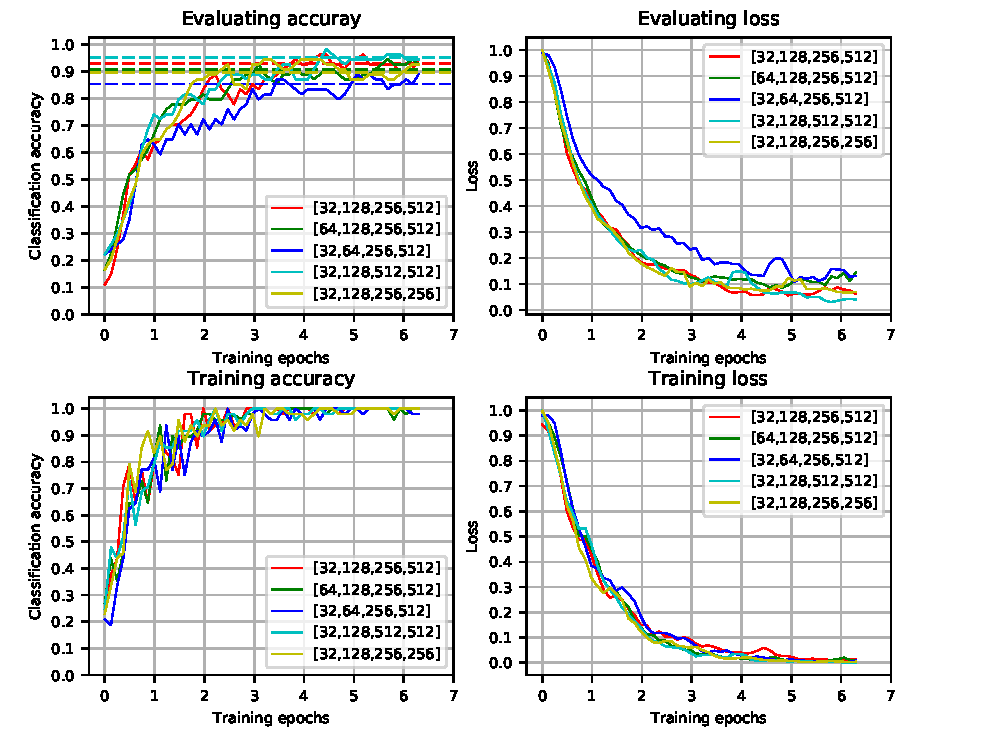
\includegraphics[trim=0cm 0cm 0cm 0cm]{fig01/plot_nof.pdf}
	\caption{The loss and classification accuracy vs. training epochs comparison between networks with different number of filters in each convolutional layer.}
	\label{fig:plot_nof}
\end{figure}



%***********************************************
% The number of neurons for each fc layer
%***********************************************
\subsubsection{The number of neurons of each fully connected layer}
\paragraph{Experimental scheme}
There are two fully connected layers in our network. In this experiment, we compared the networks with different numbers of output neurons in the fully connected layers. Specifically, we compared three cases, including \([2048,2048]\), \([4096,2048]\) and \([4096,4096]\), where the numbers in the square bracket represent the number of output neurons of the fully connected layers, e.g. \([2048,2048]\) represents \(noo\_fc6 = 2048, noo\_fc7 = 2048\), \(noo\_fc6\) is the notation of the number of output neurons of the FC6 layer.

\paragraph{Experimental results and analysis}
The experimental results are shown in Figure \ref{fig:plot_noo}. According to the experimental results, we can get following conclusions:
\begin{enumerate}
	\item The network converges a littler faster with \([4096,4096]\) output neurons, while there is no obvious difference between \([2048,2048]\) and \([4096,2048]\).
	\item The network with \([4096,4096]\) output neurons also performs a little better than the networks with  \([2048,2048]\) and \([4096,2048]\) output neurons. 
\end{enumerate}
So, we  use  \([4096,4096]\) to configure the fully connected layers of the network.
 
\begin{figure}
	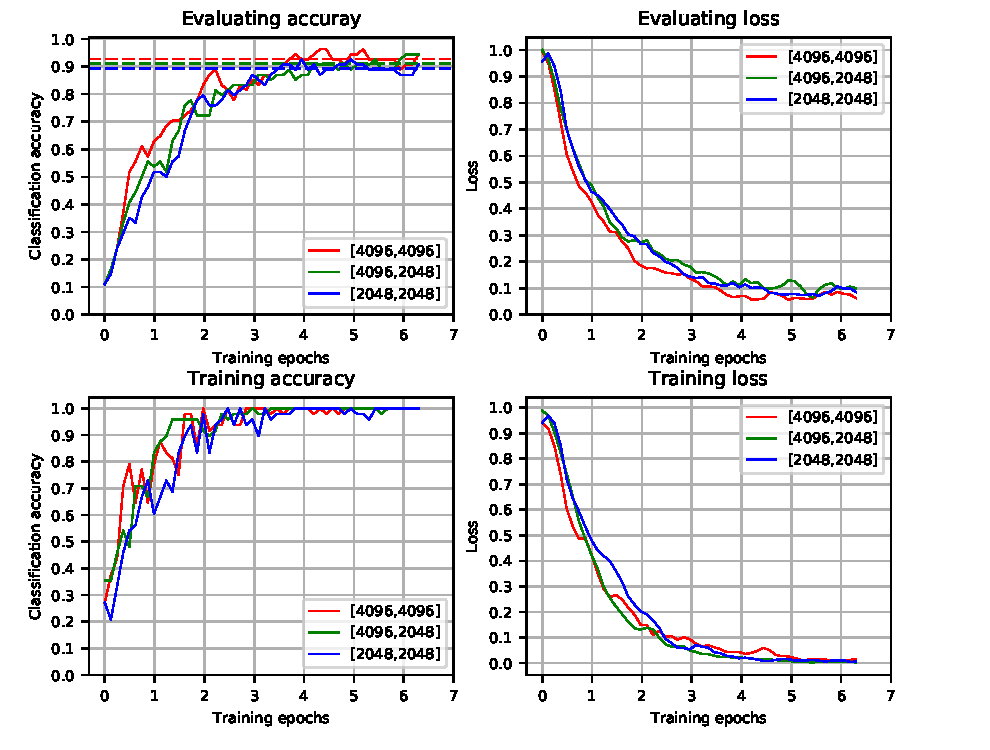
\includegraphics[trim=0cm 0cm 0cm 0cm]{fig01/plot_noo.pdf}
	\caption{The loss and classification accuracy vs. training epochs comparison between networks with different number of output neurons in each fully connected layer.}
	\label{fig:plot_noo}
\end{figure}


%***********************************************
% Data augmentation: horizontal flipping
%***********************************************
\subsubsection{Data augmentation: horizontal flipping}
\paragraph{Experimental scheme}
Horizontal flipping is a common technique to augment the training data, especially for the small scale training data, see Section \ref{pre_processing} \ref{augmentation}. We evaluated two networks trained on the data with and without horizontal flipping. 

\paragraph{Experimental results and analysis}
According to the experimental results, shown in Figure \ref{fig:plot_rlf}, the network trained on the data with horizontal flipping significant outperforms the network which is trained on the data without horizontal flipping. So, we adopt the horizontal flipping technique to augment our training data. 
\begin{figure}
	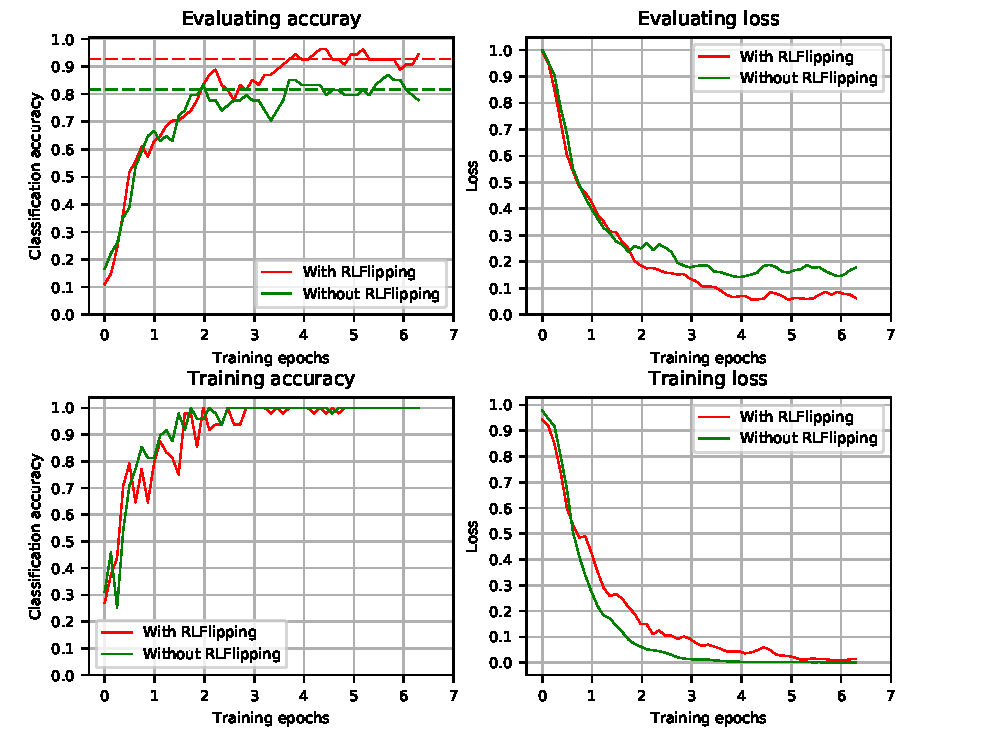
\includegraphics[trim=0cm 0cm 0cm 0cm]{fig01/plot_rlf.pdf}
	\caption{The loss and classification accuracy vs. training epochs comparison between networks trained on the data with and without horizontal flipping.}
	\label{fig:plot_rlf}
\end{figure}


%***********************************************
% Data augmentation: random cropping
%***********************************************
\subsubsection{Data augmentation: random cropping}
\paragraph{Experimental scheme}
N-time random cropping is another common used technique to augment small scale training data, see Section \ref{pre_processing} \ref{augmentation}. We evaluated three networks trained on the data with 3 different random cropping configurations, including 1-time random cropping, 2-time random cropping and 4-time random cropping. 

\paragraph{Experimental results and analysis}
The experimental results are illustrated in Figure \ref{fig:plot_rc}. According the experimental results, the random cropping technique do help much on training the network. The network trained on the data with 4-time random cropping outperforms that with 2-time random cropping, and the network trained on the data with 2-time random cropping outperforms that with 1-time random cropping. So, we use the 4-time random cropping to augment our training data in the project.
\begin{figure}
	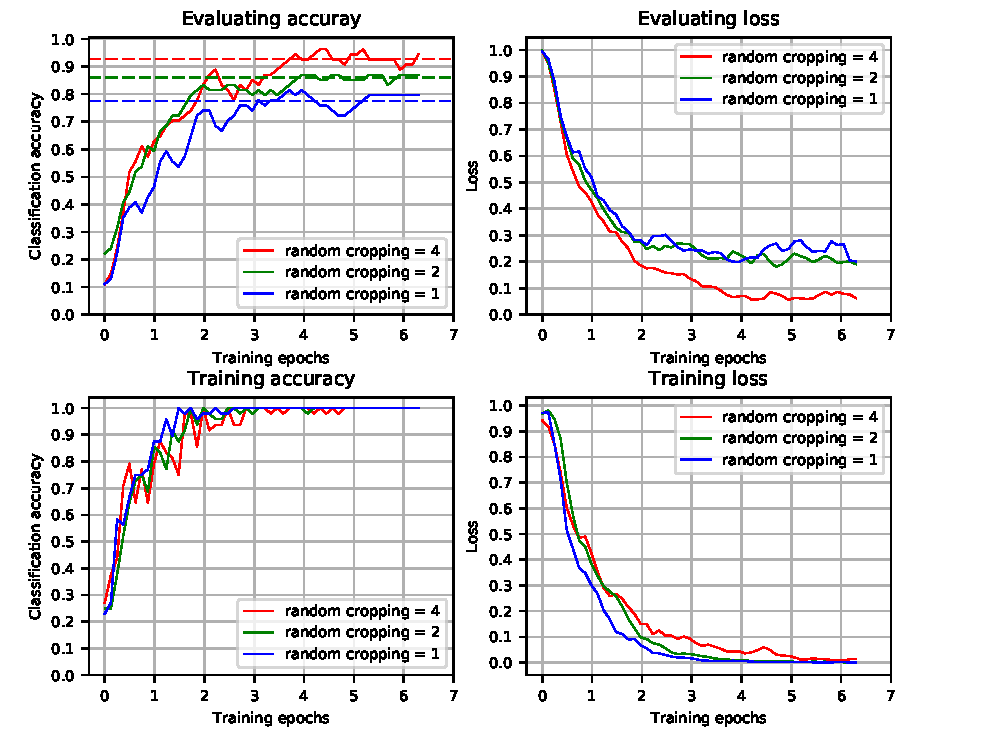
\includegraphics[trim=0cm 0cm 0cm 0cm]{fig01/plot_rc.pdf}
	\caption{The loss and classification accuracy vs. training epochs comparison between networks trained on training data with different random cropping configurations.}
	\label{fig:plot_rc}
\end{figure}


%***********************************************
% Temporal down-sampling of frames
%***********************************************
\subsubsection{Temporal down-sampling of frames}
\paragraph{Experimental scheme}
Temporal down-sampling of frames is a method which we applied to make each video clip contains more temporal information, see Section \ref{pre_processing} \ref{down-sampling}. We evaluated 4 cases: including temporal down-sampling with temporal strides 1 frame, 2 frames, 3 frames and evenly sample 16 frames from each video (temporal down-sampling = 0).  

\paragraph{Experimental results and  analysis}
The experimental results are illustrated in Figure \ref{fig:plot_tds}. The network trained on the data which are evenly sampled 16 frames from each input video performs the best. And the other three network have similar performance. So, we set temporal down-sampling mode to 0 to pre-process our training data.
\begin{figure}
	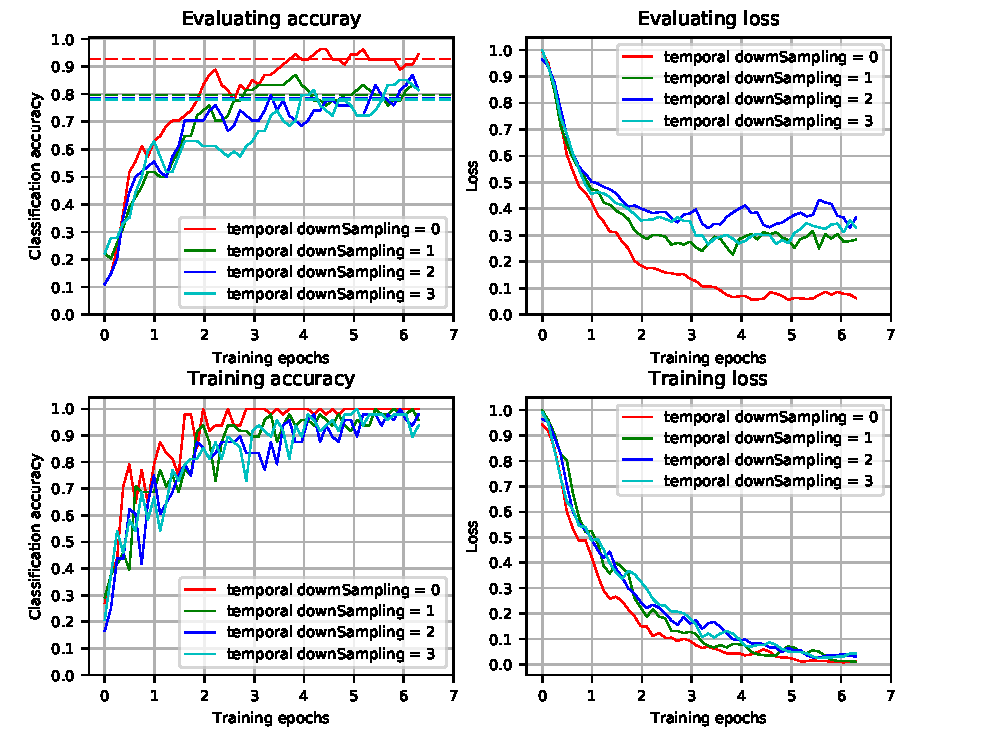
\includegraphics[trim=0cm 0cm 0cm 0cm]{fig01/plot_tds.pdf}
	\caption{The loss and classification accuracy vs. training epochs comparison between networks trained on training data with different temporal down-sampling strides.}
	\label{fig:plot_tds}
\end{figure}


%***********************************************
% Data normalization
%***********************************************
\subsubsection{Data normalization}
\paragraph{Experimental scheme}
Normalizing the data before feeding to the network is a common method, see Section \ref{pre_processing} \ref{normalization}. In this experiment, we evaluated three different data normalization methods, including: 1). directly scale the value of \(X\) from \(0-255\) to \(0-1\), 2), subtract the \(mean\) value (\(X-mean\)),  3), subtract the mean value and divide it by the stand deviance value (\((X-mean)/std\)).   
\paragraph{Experimental results and analysis}
The experimental results are illustrated in Figure \ref{fig:plot_dnm}. According to the experimental results, the network trained on the data with normalization mode (\(X -mean\)) performs best among the three, and the other two networks have similar performance. So, we use the normalization mode (\(X -mean\)) to normalize the data in our project.
\begin{figure}
	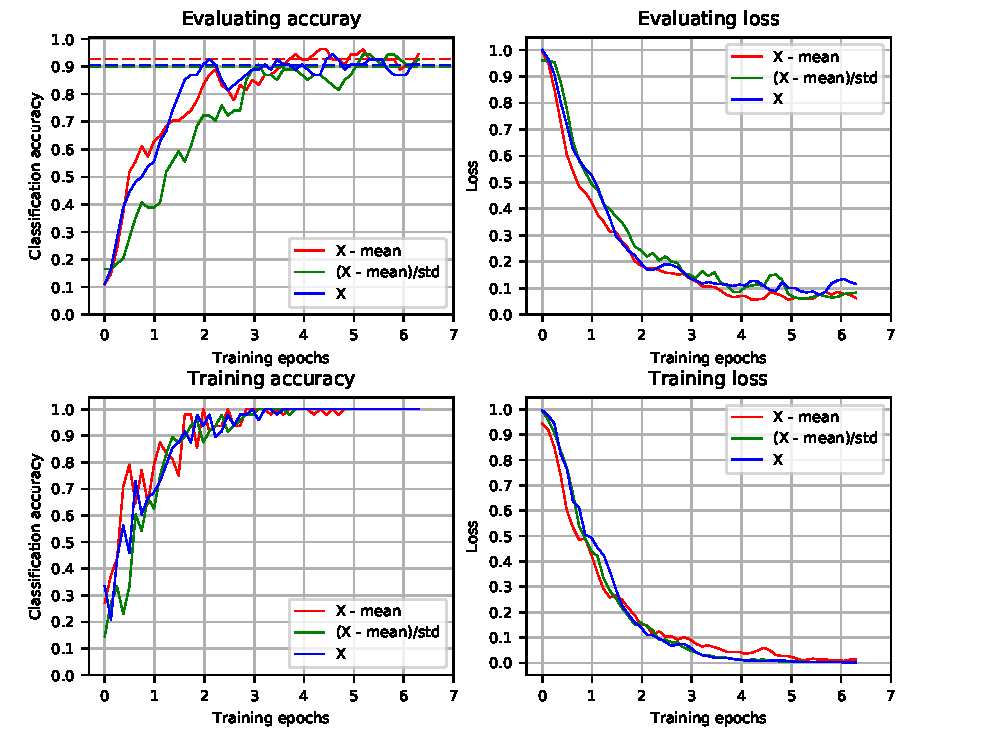
\includegraphics[trim=0cm 0cm 0cm 0cm]{fig01/plot_dnm.pdf}
	\caption{The loss and classification accuracy vs. training epochs comparison between networks trained on training data with different normalization methods.}
	\label{fig:plot_dnm}
\end{figure}

\subsection{Conclusions of parameter searching}
According to all of the above experiments which we performed for parameter searching, we can get following conclusions:
\begin{enumerate}
	\item In the network side,  the factors which affect the performance much are not the architecture or the hyper-parameters of the network but those factors in the training processing, including the initialization of network parameters, learning rate and the keep probability of the dropout layers. 
	\item In the data pre-processing side, almost all factors except the data normalization method affect the performance of the network much.  Such conclusion also indicates that the data is the critical factor of our project.   
\end{enumerate}

\section{The experimental results of of the interaction classification}
\subsection{Train the network from scratch}
\subsubsection*{Experimental scheme}
In this step, we train the fullNet on UT-Interaction dataset from scratch. We face a new problem when we try to apply all optimal parameter settings from singleNet to fullNet. That is the overall GPU memory allocation requirement for the fullNet is larger than 24GiB which is beyond the GPU resource we have in hand. So, we slightly adjust the hyper-parameters of the fullNet. The adjusted hyper-parameters are the values of \(noo\_fc5\) and \(noo\_fc6\) , and both from \(4096\) to \(2048\). To compare the performance between the fullNet and singleNet, we build three models: a). fullNet with adjusted hyper-parameters notated as fullNet\_2048, b). singleNet with optimal hyper-parameters notated as singleNet\_4096, and c). singleNet with adjusted hyper-parameters notated as singleNet\_2048.  The data pre-processing methods and parameter settings, the architecture and hyper-parameter settings of the network, and the training settings are illustrated in the Table \ref{table:network_settings}.
  
  \renewcommand\arraystretch{1.2}  
\begin{table}
	\caption{Parameter, network architecture and training settings for network and data pre-processing.}
	\begin{center}
		\begin{tabular}{| m{0.6cm} | m{7cm} | m{6cm} |}
			\hline
			\textbf{No.} & \textbf{Factors} & \textbf{Parameters}  \\ \hline \hline
			% Network
			\multicolumn{3}{|l|}{\textbf{Network}}  \\ \hline
			
			1 & Initial values of the network parameters, see Section \ref{Initialization}. & \tabincell{l} 
			{ \(weights\) : "Xavier" initialization \\ 
				\(biases\) : constant 0.1} \\ \hline
			
			2 & Dynamic adjusting of the learning rate, see Section \ref{learning_rate}. & \(Learning\ rate = 1e^{-4} \)	\\ \hline
			
			3 & Dropout layers, see Section \ref{dropout} & \(keep\_ratio = 0.5\)	\\ \hline
			
			4 & Batch normalization layers, see Section \ref{bn} &  Yes  \\ \hline
			
			5 & The number of convolutional layers, see Section \ref{3dconv_layers} & 5\\ \hline
			
			6 & The size of convolutional kernels, see Section \ref{3dconv_filters} & \(3 \times 3 \times 3\) \\ \hline
			
			7 & The sizes of the pooling kernels, see Section \ref{3dconv_filters} & \tabincell{l}
			{L1: \(1 \times 2 \times 2 \) \\ 
				L2, L3, L4: \(2 \times 2 \times 2 \) \\
				L5: \(2 \times 1 \times 1 \)}   \\ \hline
			
			8 &  The number of filters for each convolutional layer, see Section \ref{3dconv_filters} &  \tabincell{l}
			{nof\_conv1 = 32 \\ 
			nof\_conv2 = 128  \\
			nof\_conv3 = 256  \\
			nof\_conv4 = 512 \\
			nof\_conv5 = 512}  \\ \hline
			
			9 &  The number of output neurons for each fully connected layer, see Section \ref{fc} & \(\text{noo\_fc}_*\) = 4096 \\ \hline \hline                           
			
			% Network
			\multicolumn{3}{|l|}{\textbf{Data pre-processing}}  \\ \hline
			1 & Data augmentation: horizontal flipping, see Section \ref{pre_processing} \ref{augmentation} & Yes  \\ \hline
			2 & Data augmentation: random cropping, see Section \ref{pre_processing} \ref{augmentation} & Yes, 4 times \\ \hline
			3 & Temporal down-sampling of frames, see Section \ref{pre_processing} \ref{down-sampling} & Yes, N=0, see \ref{down-sampling} \\ \hline
			
			4 & Data normalization, see Section \ref{pre_processing} \ref{normalization} & Yes, \(X_i = X_i - Mean(X)\) \\ \hline			
		\end{tabular}
		\label{table:network_settings}
	\end{center}
\end{table} 
\subsubsection*{Experimental results}
The classification accuracy for these three models are illustrated in Table \ref{table:threeModels}.

\begin{table}
	\caption{The experimental results of the three models' classification accuracy, evaluated on UT-Interaction set1}
	\begin{center}
		\begin{tabular}{| m{4cm} | m{4cm} |}
			\hline
			Model & Classification Accuracy \\ \hline \hline
			fullNet\_2048 & 87.4\%   \\ \hline
			singleNet\_4096 & 88.8\% \\ \hline
			singleNet\_2048 & 75.6\%  \\ \hline				
		\end{tabular}
		\label{table:threeModels}
	\end{center}
\end{table}

\section{The experimental results of of the interaction detection}
The goal of interaction detection in UT-Interaction is to locate interactions spatially and temporally in a given un-segmented video which contains 6 interactions in each single video. Since the performance of interaction detection is highly dependent on the quality of  the interacting people detection. So, we fist introduce the results of the interacting people detection, then the detail performance of the interaction detection.     

\subsection{The results of the interacting people detection}
We don't have the ground truth to report the precision-recall graph directly for the results of interacting people detection. The results are illustrated in Figure \ref{fig:int_det} with bounding boxes annotated for set1. The sequences 1 to 4 are easy since there are only two interacting people appear in the scene, but it is more challenge to locate the positions of interacting people for sequences 5 to 10, because both interacting people and irrelevant pedestrians are present in scene. We adopt the method mentioned in the previous chapter \ref{locate_interacting_people} to exclude the irrelevant people. From the results in Figure \ref{fig:int_det}, we successfully locate the spatial positions of interacting people for all videos except the sequence 9, because the relative position between the irrelevant people are very close to the target interacting people and they execute the activities simultaneously.  
\begin{figure}
	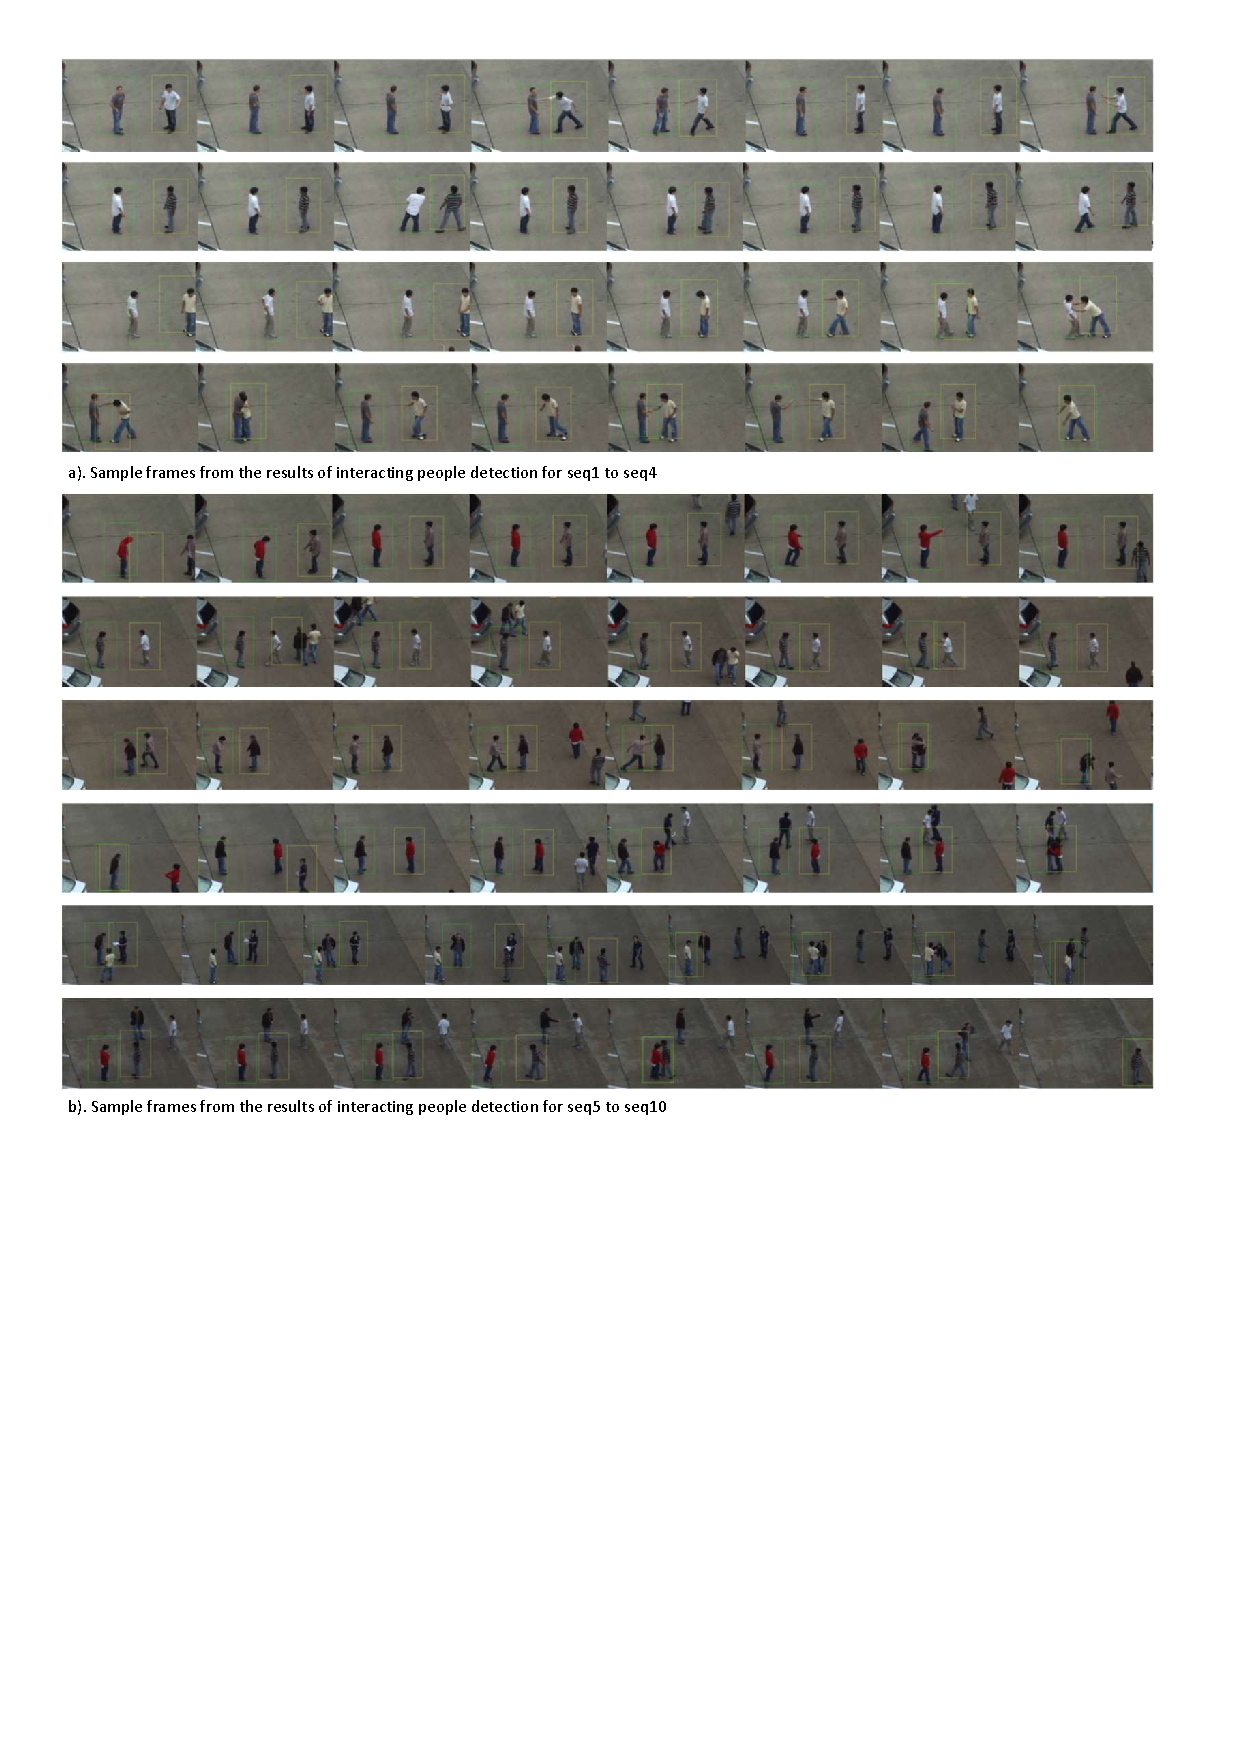
\includegraphics[trim=2cm 10.5cm 0cm 1cm]{fig01/interacting_person_det.pdf}
	\caption{Sample frames of the results of interacting people detection}
	\label{fig:int_det}
\end{figure}
 
\subsection{The results of interaction detection}
Due to classification accuracy of the singleNet\_4096 is slightly better than that of fullNet\_2048, we choose the trained singleNet\_4096 as the feature descriptor for the interaction detection task.

\textcolor[rgb]{0,0,1}{\textit{\large The results of interaction detection need to be added here}}.
\\
\par

\section{Discussion}
%=========================================================